\documentclass[12pt, a4paper]{article}

\usepackage[T1]{fontenc}
\usepackage{courier}
\usepackage{graphicx}
\usepackage{caption}
\usepackage{mathptmx}
\usepackage{ragged2e}
\usepackage{xcolor}
\usepackage{listings}
\usepackage{enumitem}

\graphicspath{{img}}
\pagenumbering{gobble}
\date{}

\captionsetup[figure]{labelformat=empty}

\title{

  \LARGE{\textbf{LAPORAN}}

  {\vspace{1cm}}

  \large{\textbf{Eksplorasi Pembuatan Simulasi Server Topologi Hybrid}}

  {\large{Diajukan untuk Memenuhi Tugas Mata Kuliah Jaringan Komputer}}

  {\vspace{1cm}}

  \normalsize{Radinal Shidiq Saragih}

  \normalsize{FOO}

  \normalsize{FOO}

  {\vspace{1cm}}

  {
\includegraphics[scale=1.8]{LogoFakultas.jpeg}}

  {\vspace{2cm}}

  {\large{PROGRAM STUDI TEKNIK INFORMATIKA}}

  {\large{FAKULTAS TEKNIK}}

  {\large{UNIVERSITAS SURYAKANCANA}}

  {\large{CIANJUR}}

  {\small{2024}}
}

\begin{document}
  \begin{titlepage}
    \maketitle
  \end{titlepage}

  \pagenumbering{roman}

  \begin{center}
    \section*{KATA PENGANTAR}
  \end{center}

  \setcounter{section}{1}

  \setcounter{subsection}{0}

  \addcontentsline{toc}{section}{KATA PENGANTAR}{}


  \vspace{1cm}

  FOOBAR

  \vspace{1cm}

  \begin{flushright}
    Cianjur, Oktober 2024

    \vspace{0.5cm}

    Penulis
  \end{flushright}

  \newpage

  \renewcommand\contentsname {\Large{\textbf{DAFTAR ISI}} }

  \begin{center}
  \tableofcontents
  \end{center}
  \addcontentsline{toc}{section}{DAFTAR ISI}{}

  \newpage
  
  \pagenumbering{arabic}

%---------------------------------------------------------------------------

  \begin{center}
    \large{\textbf{BAB I}}

    \section*{PENDAHULUAN}
  \end{center}
  \addcontentsline{toc}{section}{BAB I PENDAHULUAN}{}
  \vspace{1cm}
  \setcounter{section}{1}
  \setcounter{subsection}{0}


    \subsection{Latar Belakang}

    FOO

    \subsection{Rumusan Masalah}

      Adapun rumusan masalah yang akan dibahas dalam laporan ini, antara lain

      \begin{enumerate}[label=\arabic*.]
        \item Apa 
        \item Apa 
        \item Apa 
        \item Apa
      \end{enumerate}

    \subsection{Tujuan}

      Adapun yang menjadi tujuan dari laporan ini, yaitu

      \begin{enumerate}[label=\arabic*.]
        \item FOO
        \item FOO
        \item FOO
      \end{enumerate}

  \newpage

%---------------------------------------------------------------------------

  \begin{center}
    \large{\textbf{BAB II}}

    \section*{ANALISIS DAN DESIGN}
  \end{center}
  \addcontentsline{toc}{section}{BAB II ANALISIS DAN DESIGN}{}
  \vspace{1cm}
  \setcounter{section}{2}
  \setcounter{subsection}{0}

  \subsection{Desain Topologi}

  \begin{figure}[h]
      \centering
      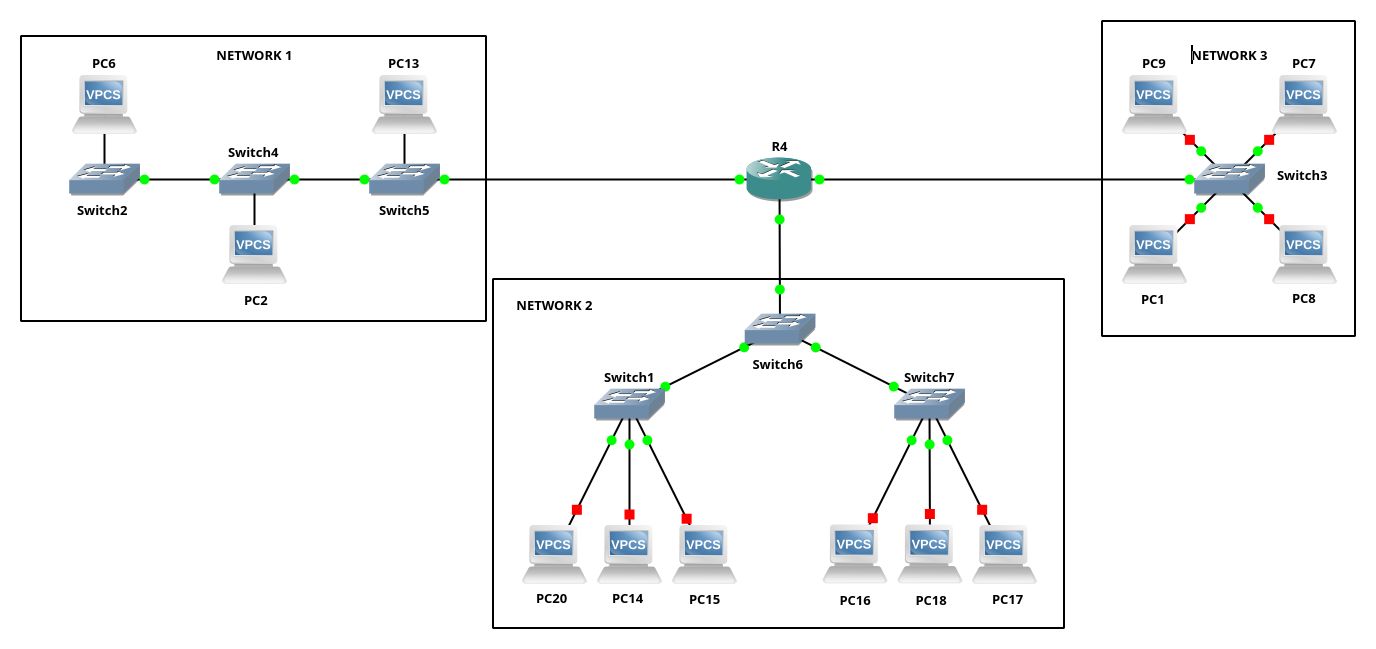
\includegraphics[scale=0.30]{TOPOLOGIBASE.png}
      \caption{\small{Bentuk Topologi}}
  \end{figure}

  Topologi di dalam simulasi ini terdiri dari tiga jaringan komputer,
  yang terhubung dengan satu sama lain melalui sebuah router.Penggunaan router untuk penghubung
  antar jaringan memungkinkan fleksibilitas dalam mengelola lalu
  lintas data antar jaringan. ketiga jaringan yang terhubung ke router masing-masing
  memiliki topology yang berbeda, yaitu.

  \begin{enumerate}
    \item Topologi Bus (Network 1)
    \item Topologi Tree (Network 2)
    \item Topologi Star (Network 3)
  \end{enumerate}

  Di ketiga jaringan tersebut akan memiliki setidaknya tiga
  VPCS (Komputer Virtual) yang semuanya terhubung ke sebuah konsentrator.
  Switch sebagai konsentrator akan lebih efektif dibandingkan hub karena
  kemampuannya dalam mengelola aliran data secara lebih efisien.
  Switch dapat menghindari terjadinya collision, karena dapat menyebabkan
  penurunan kinerja jaringan secara signifikan, seperti peningkatan latensi dan
  packet loss rate. Dan dengan Switch dapat juga menyediakan opsi konfigurasi
  yang lebih beragam dibandingkan Hub, semisalnya untuk menggunakan 
  sistem tagging VLAN semisalnya.


  \subsection{Analisis Kebutuhan}

  Seluruh perangkat yang terhubung dalam simulasi jaringan komputer ini akan
  berbentuk virtual, berikut adalah perangkat virtual yang digunakan.

  \begin{enumerate}
    \item Router Cisco (Seri 3700-an)

      Router Cisco yang digunakan akan memerlukan
      setidaknya 3 koneksi Ethernet, agar dapat
      menghubungkan semua jaringan dalam simulasi. Dan karena 
      hanya memerlukan fitur paling dasar dari sebuah router Cisco,
      disini model seri 3700 akan digunakan.

    \item GNS3 Switch

      Switch yang digunakan adalah switch default GNS3, karena beberapa alasan
      yaitu pertama untuk di simulasi ini tidak akan ada konfigurasi rumit
      kepada Switch, dan juga jauh lebih hemat memory RAM dan CPU dibandingkan
      menggunakan sebuah Switch yang di-virtualisasi ataupun EtherSwitch yang
      merupakan sebuah router cisco yang di konfigurasi agar bekerja selayaknya
      switch ethernet.

    \item VPCS (PC Virtual)

      VPCS digunakan sebagai representasi perangkat user yang terhubung pada
      jaringan, tugas nya hanya satu yaitu untuk mesimulasikan aktifitas user.

      VPCS digunakan disini dibandingkan sebuah VM (Virtual Machine) karena
      penggunaaan sumber daya yang lebih kecil

  \end{enumerate}

  \newpage

  \subsection{Konfigurasi Jaringan}

  Untuk dapat membuat semua perangkat yang terhubung dapat berkomunikasi,
  perlu untuk tiap perangkat agar memiliki alamat IP masing-masing.

  Ditabel berikut telah dilampirkan konfigurasi yang akan digunakan,

  \begin{figure}[h]
      \centering
      \begin{tabular}{|c|c|c|c|c|c|}
        \hline
        NAMA & TIPE & INTERFACE & IP & MASK & GATEWAY \\
        \hline
        R1 & Router & FastEthernet0/0 & 192.168.1.1 & 255.255.255.0 & - \\
        \hline
        R1 & Router & FastEthernet0/1 & 192.168.2.1 & 255.255.255.0 & - \\
        \hline
        R1 & Router & FastEthernet1/0 & 192.168.3.1 & 255.255.255.0 & - \\
        \hline
        PC6 & VPCS & Ethernet0 & 192.168.1.10 & 255.255.255.0 & 192.168.1.1 \\
        \hline
        PC2 & VPCS & Ethernet0 & 192.168.1.20 & 255.255.255.0 & 192.168.1.1 \\
        \hline
        PC13 & VPCS & Ethernet0 & 192.168.1.30 & 255.255.255.0 & 192.168.1.1 \\
        \hline
        PC20 & VPCS & Ethernet0 & 192.168.2.10 & 255.255.255.0 & 192.168.2.1 \\
        \hline
        PC14 & VPCS & Ethernet0 & 192.168.2.20 & 255.255.255.0 & 192.168.2.1 \\
        \hline
        PC15 & VPCS & Ethernet0 & 192.168.2.30 & 255.255.255.0 & 192.168.2.1 \\
        \hline
        PC16 & VPCS & Ethernet0 & 192.168.2.40 & 255.255.255.0 & 192.168.2.1 \\
        \hline
        PC18 & VPCS & Ethernet0 & 192.168.2.50 & 255.255.255.0 & 192.168.2.1 \\
        \hline
        PC17 & VPCS & Ethernet0 & 192.168.2.60 & 255.255.255.0 & 192.168.2.1 \\
        \hline
        PC9 & VPCS & Ethernet0 & 192.168.3.10 & 255.255.255.0 & 192.168.3.1 \\
        \hline
        PC7 & VPCS & Ethernet0 & 192.168.3.20 & 255.255.255.0 & 192.168.3.1 \\
        \hline
        PC1 & VPCS & Ethernet0 & 192.168.3.30 & 255.255.255.0 & 192.168.3.1 \\
        \hline
        PC8 & VPCS & Ethernet0 & 192.168.3.40 & 255.255.255.0 & 192.168.3.1 \\
        \hline
      \end{tabular}
      \caption{\small{Tabel Konfigurasi IP}}
  \end{figure}

  Pada dasarnya hanya terdapat dua tipe perangkat pada jaringan ini yang
  memerlukan konfigurasi IP, yaitu perangkat VPCS (komputer virtual) dan
  juga sebuah router, tepatnya router Cisco 3725. Jadi pada bagian ini, akan
  ditampilkan langkah-langkah untuk mengkonfigurasi kedua tipe perangkat 
  tersebut.

  Perangkat pertama yang harus didahulukan untuk dikonfigurasi adalah router,
  karena pengaturan IP pada interface jaringan di router ini akan menentukan
  bagaimana pengaturan IP dan Gateway di semua VPCS yang ada di jaringan ini.

  \newpage

  \begin{figure}[h]
      \centering
      \includegraphics[scale=0.40]{CISCO\_CONSOLE.png}
      \caption{\small{Tampilan terminal Router Cisco}}
  \end{figure}

  Untuk mengkonfigurasi sebuah router Cisco dapat dilakukan melalui interface
  terminal, disana akan terdapat berbagai perintah-perintah untuk menentukan
  bagaimana router berkerja.

  Hal pertama yang perlu dilakukan  adalah untuk melihat terlebih dahulu
  interface yang tersedia pada router, untuk melihat semua interface yang
  tersedia serta status terkini dari interface tersebut, dapat melalui 
  perintah berikut.

  \begin{figure}[h]
      \centering
      \includegraphics[scale=0.40]{CISCO\_SHOW\_INTERFACE.png}
      \caption{\small{Daftar Interface Yang Tersedia serta Statusnya}}
  \end{figure}

  Di tampilan tersebut dapat dilihat bahwa terdapat 4 buat interface yang dapat
  digunakan di router ini, dan semuanya masih dalam kondisi down atau tidak
  aktif serta belum memiliki alamat IP.

  Pengaturan pada router cisco dilakukan melalui sebuah
  mode konfigurasi, yang dapat dilihat pada gambar berikut.

  \begin{figure}[h]
      \centering
      \includegraphics[scale=0.50]{CISCO\_CONFIG\_TERMINAL.png}
      \caption{\small{Tampilan Mode Konfigurasi}}
  \end{figure}

  pada gambar tersebut, terdapat beberapa perintah. Pertama ``enable`` yang
  merupakan perintah untuk membuka opsi konfigurasi adminstrator. Lalu
  perintah ``config terminal`` yang merupakan perintah untuk membuka mode
  konfigurasi.

  Untuk memberikan sebuah alamat IP kepada suatu interface, dapat dilakukan
  dalam mode konfigurasi dengan perintah-perintah sebagai berikut.

  \begin{figure}[h]
      \centering
      \includegraphics[scale=0.40]{CISCO\_CONFIG\_INTERFACE.png}
      \caption{\small{Pengaturan IP pada Interface}}
  \end{figure}

  Pada gambar diatas, terdapat empat command, yaitu.

  \begin{enumerate}
    \item ``interface FastEthernet0/0``

      Perintah ini mengatakan bahwa kita ingin melakukan perubahan terhadap 
      pengaturan pada interface yang bernama ``FastEthernet0/0``, setelah
      perintah ini dijalankan, semua konfigurasi setelahnya akan diterapkan
      pada tingkat interface yang tadi dipilih saja.

    \item ``ip address 192.168.1.1 255.255.255.0``

      Perintah ini menyatakan kita ingin memberikan alamat IP ``192.168.1.1``
      dengan subnet mask yaitu 255.255.255.0.

    \item ``no shutdown``

      Perintah ini mengatakan bahwa kita ingin interface ``FastEthernet0/0``
      yang dipilih tadi untuk diaktifkan, dan tetap aktif.

    \item ``end``

      Perintah ini akan mengeluarkan anda dari mode konfigurasi, kembali
      ke mode sebelumnya.

  \end{enumerate}

  \newpage

  Setelah melakukan langkah-langkah diatas, interface akan diaktifkan serta diberi
  alamat IP. Lakukan hal yang sama untuk semua interface yang akan digunakan
  pada topologi ini, hingga daftar status dan IP yang sebelumnya berubah
  menjadi sebagai berikut.

  \begin{figure}[h]
      \centering
      \includegraphics[scale=0.40]{CISCO\_SHOW\_INTERFACE\_DONE.png}
      \caption{\small{Daftar Interface Yang Sudah Di Konfigurasi}}
  \end{figure}

  Setelah Router terkonfigurasi, yang perlu dilakukan sekarang hanya 
  mengkonfigurasi tiap vpcs yang terhubung pada jaringan alamat-alamat IP serta
  gateway yang sesuai. Alamat gateway menyatakan bahwa VPCS tersebut akan
  berkomunikasi melalui alamat IP tersebut, biasanya gateway adalah alamat
  suatu interface seperti yang ada pada router tadi. Gunakan tabel konfigurasi IP
  yang sebelumnya telah disajikan untuk refrensi.

  Untuk mengkonfigurasi VPC dapat dilakukan dengan mudah, melalui
  konsol seperti sebagai berikut.
  
  \begin{figure}[h]
      \centering
      \includegraphics[scale=0.40]{CONFIG\_VPCS.png}
      \caption{\small{Konfigurasi alamat IP serta Gateway VPCS}}
  \end{figure}

  Disini VPCS PC6 dikonfigurasi untuk menggunakan alamat IP 192.168.1.10 dengan
  gateway 192.168.1.1 (alamat Interface FastEthernet0/0 pada router). Yang 
  perlu diperhatikan di sini adalah nilai subnet berada pada range gateway yang
  terhubung pada jaringan dimana VPCS tersebut berada.

  Lakukan hal yang sama untuk tiap VPCS, gunakan tabel konfigurasi IP sebagai
  refrensi.

  \newpage

  Maka, pada akhir tahapan konfigurasi, tiap perangkat akan memiliki alamat-alamat
  sebagai berikut.

  \begin{figure}[h]
      \centering
      \includegraphics[scale=0.35]{TOPOLOGY\_IP.png}
      \caption{\small{Topologi dengan Semua Perangkat Terkonfigurasi}}
  \end{figure}

  \newpage

%---------------------------------------------------------------------------

  \begin{center}
    \large{\textbf{BAB III}}
    \section*{PENGUJIAN}
  \end{center}
  \addcontentsline{toc}{section}{BAB III PENGUJIAN}{}
  \setcounter{section}{3}
  \setcounter{subsection}{0}
  \vspace{1cm}

  \subsection{Metode Pengujian}
  Pengujian keberhasilan topologi yang telah dibuat sebelumnya dapat dilakukan
  dengan dengan menguji konektivitas vpcs yang berada di topologi tersebut. hal
  ini dapat dilakukan dengan mengirimkan paket-paket data melalui sebuah perintah
  terminal pada VPCS yaitu, ``ping``.

  Perintah terminal ``ping`` akan pertama mengirimkan sebuah permintaan atau
  \emph{request} ICMP (Internet Control Message Protocol) ke sebuah mesin di
  alamat IP tujuan, dan mesin yang dikirimkan permintaan tersebut akan merespon
  dengan sebuah balasan atau \emph{reply}. dengan ini sebagai pertanda bahwa
  sebuah mesin dapat berkomunikasi dengan mesin yang dituju adalah adanya 
  kedua respon yang telah disebut sebelumnya.

  Pengujian pada topologi ini menghubungkan sekitar tiga belas (13) buah
  VPCS hanya tiga buah VPCS dari tiga jaringan berbeda yang akan digunakan
  dalam proses pengujian, karena dari segi pengalamatan semua VPCS hanya
  ada tiga subnet dan getway yang berbeda, hingga tiap VPCS tersebut
  sudah dapat mewakili konektivitas untuk tiap jaringan yang terhubung
  pada topologi ini.

  Ketiga VPCS dari ketiga jaringan tersebut akan diuji ``ping`` terhadap
  mesin yang ada di kedua jaringan lainnya. Misalkan satu VPCS pada 
  Network 1 maka akan diuji pada Network 2 dan 3.

  \newpage

  \subsection{Pengujian Ping}

  Berikut adalah pengujian konektivitas dari VPCS PC6, PC20, dan PC1 yang
  berturut turut berada pada Network 1, 2, dan 3.

  \begin{enumerate}

    \item PC6 (Network 1) (192.168.1.10)
      \begin{enumerate}
        \item Ke PC20 (192.168.2.10)
          \begin{figure}[h]
              \centering
              \includegraphics[scale=0.50]{PC6\_T1.png}
              \caption{\small{Ping PC6 ke PC20}}
          \end{figure}
        \item Ke PC1 (192.168.3.30)
          \begin{figure}[h]
              \centering
              \includegraphics[scale=0.50]{PC6\_T2.png}
              \caption{\small{Ping PC6 ke PC1}}
          \end{figure}
      \end{enumerate}

    \item PC20 (Network 2) (192.168.2.10)
      \begin{enumerate}
        \item Ke PC6 (192.168.1.10)
          \begin{figure}[h]
              \centering
              \includegraphics[scale=0.50]{PC20\_T1.png}
              \caption{\small{Ping PC20 ke PC6}}
          \end{figure}

    \newpage

        \item Ke PC1 (192.168.3.30)
          \begin{figure}[h]
              \centering
              \includegraphics[scale=0.50]{PC20\_T2.png}
              \caption{\small{Ping PC20 ke PC1}}
          \end{figure}
      \end{enumerate}

    \item PC1 (Network 3) (192.168.3.30)
      \begin{enumerate}
        \item Ke PC6 (192.168.1.10)
          \begin{figure}[h]
              \centering
              \includegraphics[scale=0.50]{PC1\_T1.png}
              \caption{\small{Ping PC1 ke PC6}}
          \end{figure}
        \item Ke PC20 (192.168.2.10)
          \begin{figure}[h]
              \centering
              \includegraphics[scale=0.50]{PC1\_T2.png}
              \caption{\small{Ping PC1 ke PC20}}
          \end{figure}
      \end{enumerate}

  \end{enumerate}

  \newpage

%---------------------------------------------------------------------------

  \begin{center}
    \large{\textbf{BAB IV}}
    \section*{KESIMPULAN}
  \end{center}
  \addcontentsline{toc}{section}{BAB IV KESIMPULAN}{}
  \setcounter{section}{4}
  \setcounter{subsection}{0}
  \vspace{1cm}

  \newpage

%---------------------------------------------------------------------------

  \begin{center}
    \section*{DAFTAR PUSTAKA}
  \end{center}
  \addcontentsline{toc}{section}{DAFTAR PUSTAKA}{}
  \vspace{1cm}

  \begin{enumerate}
    \item FOO
    \item FOO
  \end{enumerate}

%---------------------------------------------------------------------------


\end{document}
